\documentclass[11pt,a4paper,twoside,openright]{memoir}


%%% PREAMBULES %%%
\usepackage[utf8]{inputenc}
\usepackage[T1]{fontenc}


% POLICES
\usepackage{lmodern} % lmodern pour le mode math...
\edef\oldtt{\ttdefault} % et le mode typewriter
\usepackage[oldstyle, proportional]{libertine} % libertine comme police principale
\renewcommand{\ttdefault}{\oldtt}
\usepackage[scaled=0.875]{helvet} % helvetica comme police sans serif
\usepackage{slantsc} % slanted small caps

% preambules
% Page layout (margins)
%\usepackage[margin=28mm,includeheadfoot,bindingoffset=5mm]{geometry}

\settrimmedsize{297mm}{210mm}{*}
\setlength{\trimtop}{0pt} 
\setlength{\trimedge}{\stockwidth} 
\addtolength{\trimedge}{-\paperwidth} 

% si no de page en bas
% \setlrmarginsandblock{3.25cm}{*}{*} % spine, edge, edge-to-spine ratio
% \setulmarginsandblock{3.0cm}{*}{1.25} % upper, lower, lower-to-upper ratio
% \setheadfoot{\onelineskip}{2\onelineskip}
% \checkandfixthelayout 


% si no de page en haut
\setlrmarginsandblock{3.2cm}{*}{*} % spine, edge, edge-to-spine ratio
\setulmarginsandblock{3.0cm}{*}{} % upper, lower, lower-to-upper ratio
\setheadfoot{\onelineskip}{\onelineskip}
\checkandfixthelayout 


% Show page margins, \usepackage[noframe]{showframe} to disable
\usepackage[noframe]{showframe}
%https://tex.stackexchange.com/questions/328662/showframe-how-to-make-colored-lines-of-page-layout
\renewcommand*\ShowFrameColor{\color{red}} % marges
\usepackage{color,xcolor}

%\colorlet{mydarkgray}{black!84}
\definecolor{mydarkgray}{HTML}{212131}%111122}

\definecolor{DodgerBlue3}{rgb}{0.094, 0.455, 0.804}
\definecolor{bleuONERA1}{rgb}{0.09,0.40,1.00} % Bleu du logo Onera
\definecolor{bleuONERA2}{rgb}{0.0,0.33,0.66}  % Bleu de la gauche du bandeau haut
\definecolor{bleuONERA3}{rgb}{0.85,0.90,0.95} % Bleu de la droite du bandeau haut

\definecolor{deepblue}{rgb}{0.0, 0.212, 0.596}

\definecolor{myred}{rgb}{0.8431,0.1882,0.1529}
\definecolor{mygreen}{rgb}{0.2118,0.6118,0.0235}


\definecolor{redlink}{HTML}{CD463C}
\definecolor{blulink}{HTML}{3C5FCC}

\definecolor{greenlink}{HTML}{198C32}



%%%%%%%%%
\definecolor{sunset01}{HTML}{364B9A}
\definecolor{sunset02}{HTML}{4A7BB7}
\definecolor{sunset03}{HTML}{6EA6CD}
\definecolor{sunset04}{HTML}{98CAE1}
\definecolor{sunset05}{HTML}{C2E4EF}
\definecolor{sunset06}{HTML}{EAECCC}
\definecolor{sunset07}{HTML}{FEDA8B}
\definecolor{sunset08}{HTML}{FDB366}
\definecolor{sunset09}{HTML}{F67E4B}
\definecolor{sunset10}{HTML}{DD3D2D}
\definecolor{sunset11}{HTML}{A50026} % couleurs prédéfinies
%https://tex.stackexchange.com/questions/50747/options-for-appearance-of-links-in-hyperref
\usepackage[pagebackref]{hyperref} % hyper link to page where reference is cited
\renewcommand*{\backrefsep}{, }
\renewcommand*{\backreflastsep}{ et }
\renewcommand*{\backreftwosep}{ et }
\renewcommand*{\backref}[1]{}
\renewcommand*{\backrefalt}[4]{%
    \ifcase #1 {\color{red}(Pas cité)}%\relax%
    \or        (\cf p.~#2)%
    \else      (\cf pp.~#2)%
    \fi}

\hypersetup{
	breaklinks,
	colorlinks=true,
	linkcolor=DodgerBlue3,
	anchorcolor=myred,%DarkRed,%
    citecolor=DodgerBlue3,%redlink,%black,%mygreen,
	pdfdisplaydoctitle=true,
	pdfpagemode=UseOutlines,%
	bookmarksnumbered=true,
	bookmarksopen=true,
	hypertexnames=true,
	linktoc=all
}
    
\usepackage{memhfixc} % Must be used on memoir document class after hyperref (?)



% Adding package bookmark improves bookmarks handling.
% More features and faster updated bookmarks.
%https://tex.stackexchange.com/questions/65544/how-to-link-table-of-contents-in-thesis-pdf
\usepackage{bookmark}


\renewcommand*{\sectionrefname}{Section~}
\renewcommand*{\chapterrefname}{Chapitre~}
\renewcommand*{\partrefname}{Partie~}
\renewcommand*{\appendixrefname}{Appendice~}
\newcommand{\algorithmautorefname}{Algorithme} % format des liens et références croisées
\usepackage{graphicx}


\usepackage{tikz}
\usetikzlibrary{calc}

\makeatletter
\newcommand{\gettikzxy}[3]{%
  \tikz@scan@one@point\pgfutil@firstofone#1\relax
  \edef#2{\the\pgf@x}%
  \edef#3{\the\pgf@y}%
}

\newcommand{\globalgettikzxy}[3]{%
  \tikz@scan@one@point\pgfutil@firstofone#1\relax
  \edef\@tempdima{\the\pgf@x}%
  \edef\@tempdimb{\the\pgf@y}%
  \global#2=\@tempdima%
  \global#3=\@tempdimb%
}

\newcommand\getwidthofnode[2]{%
    \pgfextractx{\pgf@xb}{\pgfpointanchor{#2}{east}}%
    \pgfextractx{\pgf@xa}{\pgfpointanchor{#2}{west}}% 
    \pgfmathsetlength{\pgf@xb}{\pgf@xb - \pgf@xa}%
	\global#1=\pgf@xb%
}

\newcommand\getheightofnode[2]{%
    \pgfextracty{\pgf@yb}{\pgfpointanchor{#2}{north}}%
    \pgfextracty{\pgf@ya}{\pgfpointanchor{#2}{south}}% 
    \pgfmathsetlength{\pgf@yb}{\pgf@yb - \pgf@ya}%
	\global#1=\pgf@yb%
}
\makeatother




% chemin(s) des figures
\graphicspath{{./figures/}}%,{../fig2/}}


% controle des objets flottants (figures, tables)
\renewcommand{\topfraction}{0.7}     % autorise 70% page de graphique en haut
\renewcommand{\bottomfraction}{0.5}  % autorise 50% page de graphique en bas
\renewcommand{\floatpagefraction}{0.7}
\renewcommand{\textfraction}{0.1} % TikZ, PGF, PStricks
% Math packages, notations
\usepackage{amsthm}
\usepackage{amssymb}
\usepackage{amsmath}    % amsmath equation env has funny spacing with hyperref :-( so...
\let\equation\gather \let\endequation\endgather
\usepackage{amsfonts}
\usepackage{bm}
\usepackage{mathtools}
\usepackage{stmaryrd}

%https://tex.stackexchange.com/questions/165685/subequations-and-array-in-braces
\usepackage[overload]{empheq}

\usepackage{cases}

\usepackage{esint}
\usepackage[overload]{empheq}%https://tex.stackexchange.com/questions/165685/subequations-and-array-in-braces

\usepackage{xifthen}% provides \isempty test
\usepackage{xparse}
\usepackage{xstring}

\usepackage{mathrsfs}% script (mathscr}

% *** TWEAK (NEGATIVE) SPACES *** 
%https://tex.stackexchange.com/questions/67912/large-negative-spaces
%https://tex.stackexchange.com/questions/9091/what-is-the-right-way-to-use-the-spacing-command/9092

%https://tex.stackexchange.com/questions/2783/bold-calligraphic-typeface
\DeclareMathAlphabet\matholdcal{OMS}{cmsy}{m}{n}

%https://tex.stackexchange.com/questions/247531/how-to-use-boondox-calligraphic-font-in-latex-without-replacing-mathcal-command/247819
%https://ctan.org/pkg/mathalfa
\usepackage[
scr=boondoxo, scrscaled=1.05, 
cal=zapfc, calscaled=1.18%,
%frak=mma, frakscaled=1.,
]{mathalfa}


%https://tex.stackexchange.com/questions/399620/how-can-i-get-a-bar-over-a-subscript
\usepackage{widebar}


%https://tex.stackexchange.com/questions/234676/new-theorem-style
%https://en.wikibooks.org/wiki/LaTeX/Theorems
\newtheoremstyle%
   {mythm}% name of the style to be used
   {\topsep}% measure of space to leave above the theorem. E.g.: 3pt
   {\topsep}% measure of space to leave below the theorem. E.g.: 3pt
   {\itshape}% font to use in the body of the theorem
   {0pt}% measure of space to indent
   {\bfseries\scshape}% head font
   {~---}% punctuation between head and body
   { }%\newline}% space after theorem head; " " = normal interword space
   {}%{\thmname{#1}\thmnumber{ #2}\thmnote{ (#3)}}% Manually specify head
\theoremstyle{mythm}

\newtheorem{theoreme}{Théorème}[chapter]
\newtheorem{propriete}{Propriété}[chapter]
\newtheorem{definition}{Définition}[chapter]
\renewcommand{\proofname}{Preuve}
\renewcommand\qedsymbol{$\blacksquare$}%{C.Q.F.D.}%

% Notations
\newcommand*{\rank}[1]{\mathrm{rang}{#1}}
\newcommand*{\determinant}[1]{\det{#1}}%{\left\lvert {#1} \right\rvert}
\newcommand*{\inv}[1]{#1\raisebox{1.15ex}{$\scriptscriptstyle-\!1$}}
\newcommand*{\inverse}[1]{\ensuremath{{#1} ^{-1}}} % inverse matrix
\newcommand*{\transpose}[1]{\ensuremath{{#1} ^\mathsf{T}}} % transpose matrix
\newcommand*{\dotprod}[2]{ \transpose{#1} {#2} } % dot product
\newcommand*{\crossprod}[2]{ {#1} \times {#2} } % cross product
\newcommand*{\normtwo}[1]{ \left\| {#1} \right\| } % Euclidean norm
\newcommand*{\norminf}[1]{ \left\| {#1} \right\|_{\infty} } % infinity norm
\newcommand*{\vit}[1]{\bm{#1}} % greek letter vector
\newcommand*{\vrm}[1]{\mathbf{#1}} % latin letter vector
\newcommand*{\unitized}[1]{ \frac{#1}{\normtwo{#1}} }
\newcommand*{\scalprod}[2]{\left \langle {#1}, {#2} \right \rangle}
\newcommand*{\modulo}[1]{\pmod{#1}}%{\left[ {#1} \right]}

\DeclareMathOperator*{\argmin}{\arg\!\min} % argmin
\DeclareMathOperator*{\sign}{sign} % argmin

\newcommand*{\bigO}[1]{O\!\left( {#1} \right)} % big-O
\newcommand*{\littleo}[1]{o\!\left( {#1} \right)} % little-o

% sets
\newcommand*{\reals}{\ensuremath{\mathbb{R}}}
\newcommand*{\integers}{\ensuremath{\mathbb{N}}}
\newcommand{\family}[4]{\left\{{#1}_{#2}\right\}_{{#2}={#3},\ldots,{#4}}}
\newcommand{\ffamily}[7]{\left\{{#1}_{#2,#5}\right\}_{\substack{{#2}={#3},\ldots,{#4}\\ \substack{{#5}={#6},\ldots,{#7}}}}}
\newcommand{\polyspace}[1]{\Pi_{#1}}%\mathbb{R}_{#1}[x]}
\newcommand{\Ltwospace}{L^2\chebinterval}%\mathcal{L}_2\chebinterval}
\newcommand*{\contdiff}[1]{\ensuremath{C^{#1}}}%{\matholdcal{C}^{#1}\!}
\newcommand*{\contgeom}[1]{\ensuremath{G^{#1}}}%{\matholdcal{G}^{#1}\!}

\newcommand*{\uvdomain}{\ensuremath{\mathcal{U}}}
\newcommand*{\wdomain}{\ensuremath{\mathcal{W}}}

\newcommand*{\bx}{\vit{x}}
\newcommand*{\bu}{\vit{u}}
\newcommand*{\bd}{\vit{\delta}}
\newcommand*{\bg}{\vit{\gamma}}
\newcommand*{\bgw}{\bg_{\mkern-2muw}}
\newcommand*{\bp}{\vit{\psi}}
\newcommand*{\bpw}{\bp_{\mkern-2muw}}
\newcommand*{\bl}{\vit{\lambda}}
\renewcommand*{\bs}{\vit{\sigma}} % originally backslash in typewriter font
\newcommand*{\bsu}{\bs_{\mkern-3muu}}
\newcommand*{\bsv}{\bs_{\mkern-2muv}}
\newcommand{\bt}{\vrm{t}}
\newcommand{\br}{\vrm{r}}
\newcommand{\bo}{\vit{o}}

\newcommand*{\unv}{\vrm{n}} % unit normal vector
\newcommand*{\nv}{\hat{\unv}} % normal vector



\newcommand{\colvec}[1]{\begin{pmatrix} #1 \end{pmatrix}} % vector printed in column
\newcommand{\rowvec}[1]{ \transpose{\begin{pmatrix} #1 \end{pmatrix}} } % vector printed in row (transposed column)

% Differential operators
\newcommand*{\dfdx}[2]{\frac{\mathrm{d}}{\mathrm{d}{#2}}{#1}}
\newcommand*{\partialdfdx}[2]{\frac{\partial}{\partial{#2}}{#1}}
\newcommand*{\dkfdxk}[3]{\frac{\mathrm{d}^{#3}}{\mathrm{d}{#2}^{#3}}{#1}}
\newcommand*{\deriv}[2]{{#1}^{({#2})}}
\newcommand*{\prim}[2]{{#1}^{(\raisebox{0.2ex}{$\scriptscriptstyle-\!$}{#2})}}
\newcommand*{\jacobian}[1]{\mathbf{J}_{#1}}
\newcommand*{\gradient}[1]{\nabla \! {#1}}
\newcommand*{\hessian}[1]{\mathbf{H}_{#1}}
\newcommand*{\divergence}[1]{\nabla \cdot {#1}}%\mathrm{div}{#1}}
\newcommand*{\dx}[1]{\mathrm{d}{#1}}



% Condition number
\newcommand*{\cond}[1]{\mathrm{cond} \! \left( {#1} \right)}

% Differential geometry
\newcommand{\fff}{\mathbf{I}}     % first fundamental form
\newcommand{\sffc}{I\mkern-4.8muI} % second fundamental form coefs
\newcommand{\sff}{\mathbf{I\!I}} % second fundamental form




%% Chebyshev polynomials
% Reference interval
\newcommand*{\chebinterval}{\ensuremath{\left[ -1, 1 \right]}}
\newcommand*{\chebopeninterval}{\ensuremath{\left] -1, 1 \right[}}
\newcommand*{\series}[1]{S{#1}}
\newcommand*{\truncseries}[2]{P_{#2}{#1}}
\newcommand*{\interpolant}[2]{I_{#2}{#1}}
\newcommand*{\interpderiv}[3]{D_{#2}^{(#3)}{\!#1}}%\mathcal{D}
%\newcommand*{\interpprim}[2]{J_{#2}{#1}}
\newcommand*{\interpprim}[2]{D_{#2}^{(\raisebox{0.2ex}{$\scriptscriptstyle-\!$}1)}{\!#1}}

% Reference interval for Bernstein polynomials
\newcommand*{\berninterval}{\left[ 0, 1 \right]}

%% System of equations
\newenvironment{eqsys}
{\left\lbrace\begin{array}{@{}l@{}}}
{\end{array}\right.}
%ex :
%\begin{equation}
%	\begin{eqsys}
%		y_1 = a_1 x + b_1 \\
%		y_2 = a_2 x + b_2
%	\end{eqsys}
%\end{equation}


% Intervals
\newcommand*{\lo}[1]{\underline{#1}}
\newcommand*{\hi}[1]{\widebar{#1}}%\overline{#1}}


% GRAPHS
\DeclareMathOperator{\orig}{orig}%ine}
\DeclareMathOperator{\dest}{dest}%ination}



% ENVELOPES OF SPHERES/BALLS
%\newcommand*{\sphere}[2]{\mathscr{S}(#1,#2)}                   % sphère
\newcommand*{\spherenotation}{\mathscr{S}}
\NewDocumentCommand{\sphere}{o o}{%
	\IfValueTF{#1}{%
		\IfValueTF{#2}{%
			\ensuremath{\spherenotation(#1,#2)}%
		}{%
			\ensuremath{\spherenotation(#1)}%
		}%
	}{%
		\ensuremath{\spherenotation}%
	}%
}

\newcommand*{\ball}[2]{\mathscr{B}(#1,#2)}                     % boule ouverte
\newcommand*{\implicitsphere}{S}                               % fonction définissant implicitement une sphère
\newcommand*{\implicitEdB}[1]{\varphi_{#1}}                    % fonction définissant implicitement une EdB
\newcommand*{\EdB}[2]{{#1}^{#2}}                               % EdB
%\newcommand*{\EoS}[2]{\widehat{\EoB{#1}{#2}}}                  % EdS
\newcommand*{\influ}{\mathscr{I}}                              % zone d'influence
\newcommand*{\influEdB}[2]{\influ^{\!#2}({#1})}                % zone d'influence sur l'EdB
%\newcommand*{\influEoS}[2]{\widehat{\influ}^{\!#2}({#1})}      % zone d'influence sur l'EdS
%\newcommand*{\properEoB}[2]{\influ_*^{\!#2}({#1})}             % EdB propre
%\newcommand*{\properEoS}[2]{\widehat{\influ}_{*}^{\!#2}({#1})} % EdS propre
\newcommand*{\eos}{\vit{e}}                                    % paramétrisation de l'EdS (propre)
\newcommand*{\dilation}[2]{{#1}_{\uparrow #2}}                 % "dilatation"

\newcommand*{\envelope}{\mathcal{E}}
\newcommand*{\EdS}[2]{{\envelope}^{#2}({#1})}                  % EdS
\newcommand*{\EdSpropre}[2]{{\envelope}_{*}^{#2}({#1})}        % EdS propre
\newcommand*{\EdSpropreplus}[2]{{\envelope}_{+}^{#2}({#1})}    % EdS propre "positive"
\newcommand*{\EdSpropremoins}[2]{{\envelope}_{-}^{#2}({#1})}   % EdS propre "négative"
\newcommand*{\pseudoEdS}[2]{\widehat{\envelope}^{#2}({#1})}    % pseudo-EdS

\newcommand*{\circlenotation}{\mathscr{C}}

% SET THEORY/TOPOLOGY
\newcommand*{\closure}[1]{\widebar{#1}}%\mathrm{cl}#1}%
\newcommand*{\interior}[1]{\mathrm{int}{#1}}%\mathring{#1}}%
\newcommand*{\boundary}[1]{\partial #1}
\renewcommand*{\complement}[1]{#1^\mathsf{C}}
\newcommand*{\neigborhood}{\mathscr{V}}



%\newcommand*{\proof}[1]{\textcolor{blue!60!green}{\textbf{Preuve : }#1$\,_\blacksquare$}}



% Encircled text
\newcommand{\pgftextcircled}[1]{                                                                    
    \setbox0=\hbox{#1}%
    \dimen0\wd0%
    \divide\dimen0 by 2%
    \begin{tikzpicture}[baseline=(a.base)]%
        \useasboundingbox (-\the\dimen0,0pt) rectangle (\the\dimen0,1pt);
        \node[circle,draw,outer sep=0pt,inner sep=0.1ex] (a) {#1};
    \end{tikzpicture}
}

 % notations mathématiques
\newboolean{titlerectangle}
\setboolean{titlerectangle}{true}

\newboolean{titlevbar}
\setboolean{titlevbar}{true}

\newboolean{titlehelpers}
\setboolean{titlehelpers}{true}

\newboolean{sansseriftitles}
\setboolean{sansseriftitles}{false}

\ifthenelse{\boolean{sansseriftitles}}{
	\def\titlefont{\sffamily}%
}
{
	\def\titlefont{\rmfamily}%
}

% Table of contents style
\renewcommand*{\contentsname}{Table of contents}
\renewcommand*{\cftchapterfont}{\titlefont\bfseries}



\maxtocdepth{subsection}

% Titles
\colorlet{colchapttl}{mydarkgray}%black}%DodgerBlue3}%



\makeatletter
\makechapterstyle{mychapterstyle}{
\setlength{\beforechapskip}{0pt}%40pt}
\setlength{\midchapskip}{0pt}%25pt}
\newlength{\afterchapskipdef}
\newlength{\afterchapskipxtra}
\setlength{\afterchapskipdef}{8\onelineskip}%60pt}%

\newif\ifNoChapNumber
\newlength{\barheight}
\newlength{\barlength}
\newlength{\ttltopskip}
\setlength{\ttltopskip}{60mm}
\setlength{\barlength}{0.37\foremargin}
\setlength{\barheight}{14mm}

\newlength{\numberheight}
\ifthenelse{\boolean{sansseriftitles}}{
	\setlength{\numberheight}{1.6\barheight}
}
{
	\setlength{\numberheight}{1.63\barheight}
}

\newlength{\yshiftchapname}
\newlength{\yshiftchapnum}
\setlength{\yshiftchapname}{-\ttltopskip + 10mm + 3.9mm}
\setlength{\yshiftchapnum}{-\ttltopskip - 0.1mm}

\newlength{\vbaryshift}
\setlength{\vbaryshift}{1.25mm}
\newlength{\vbarxshift}
\setlength{\vbarxshift}{2.5mm}
\newlength{\vbarthck}
\setlength{\vbarthck}{0.6pt}
\newlength{\vbartipthck}
\setlength{\vbartipthck}{0.15pt}

\renewcommand{\chapnamefont}{\scshape\titlefont}
\renewcommand{\chapnumfont}{\normalfont\titlefont\fontsize{\numberheight}{0mm}\selectfont}
\renewcommand{\chaptitlefont}{\normalfont\titlefont\bfseries\huge}%
\renewcommand{\printchaptername}{}%\chapnamefont\@chapapp}
\renewcommand{\chapternamenum}{}
\renewcommand{\printchapternum}{}


\renewcommand\printchaptertitle[1]{
	\begin{tikzpicture}[remember picture,overlay]
		\node[yshift=-\ttltopskip] at (current page.north east) {%
			\begin{tikzpicture}[remember picture, overlay]%
				%\node[%draw=red, dashed,%*****
				%	anchor=north east,%
				%	%yshift=\yshiftchapname,%
				%	%xshift=-\foremargin,%
				%	text width=\textwidth-\vbarxshift,%
				%	minimum height=\barheight,%
				%	align=flush right,%justify,%
				%	inner sep=0mm%
				%	]%
				%	(chapttl)%
				%	at ([xshift=-\foremargin-\vbarxshift, yshift=\yshiftchapname] current page.north east)%
				%	{\chaptitlefont\color{colchapttl}##1\par};%
				%
				%\draw[red, very thick, dotted] (chapttl.west) -- (chapttl.east);%*****
				%
				%\gettikzxy{(chapttl.south west)}{\bx}{\by}%
				%\global\afterchapskipxtra=-\by%
				%\pgfmathsetlength{\afterchapskip}{\afterchapskipdef + \afterchapskipxtra}%
				%\global\afterchapskip=\afterchapskip%
				%
				\ifNoChapNumber%
                                        \node[%draw=red, dashed,%*****
					anchor=north east,%
					%yshift=\yshiftchapname,%
					%xshift=-\foremargin,%
					text width=\textwidth,%
					minimum height=\barheight,%
					align=flush right,%justify,%
					inner sep=0mm%
					]%
					(chapttl)%
					at ([xshift=-\foremargin, yshift=\yshiftchapname] current page.north east)%
					{\chaptitlefont\color{colchapttl}##1\par};
					%\draw[black, thick]%
					%	([xshift=\vbarxshift, yshift= \vbaryshift] chapttl.north east)%
					%	--%
					%	([xshift=\vbarxshift, yshift=-\vbaryshift] chapttl.south east);%
					%\relax%
				\else%
                                        \node[%draw=red, dashed,%*****
					anchor=north east,%
					%yshift=\yshiftchapname,%
					%xshift=-\foremargin,%
					text width=\textwidth-\vbarxshift,%
					minimum height=\barheight,%
					align=flush right,%justify,%
					inner sep=0mm%
					]%
					(chapttl)%
					at ([xshift=-\foremargin-\vbarxshift, yshift=\yshiftchapname] current page.north east)%
					{\chaptitlefont\color{colchapttl}##1\par};%
					\node[%draw=blue, dashed,%*****
						anchor=north west,%west,%
						align=left,%
						xshift=2\vbarxshift,%
						inner sep=0mm%
						]%
						(chapnum)% 
						at (chapttl.north east)%(chapttl.east)%
						{\color{colchapttl}\chapnumfont\thechapter};%
					%
					%\draw[blue, very thick, dotted] (chapnum.west) -- (chapnum.east);%*****
					%
%\draw[colchapttl, line width=2\vbarthck]%thick]%
%([xshift=\vbarxshift, yshift= \vbaryshift] chapttl.north east)%
%--%
%([xshift=\vbarxshift, yshift=-\vbaryshift] chapttl.south east);%
%
\coordinate (a) at ([xshift=\vbarxshift+\vbartipthck,yshift=-\vbaryshift] chapttl.south east);
\coordinate (b) at ([xshift=\vbarxshift+\vbarthck]chapttl.east);
\coordinate (c) at ([xshift=\vbarxshift+\vbartipthck,yshift=+\vbaryshift] chapttl.north east);
\coordinate (d) at ([xshift=\vbarxshift-\vbartipthck,yshift=+\vbaryshift] chapttl.north east);
\coordinate (e) at ([xshift=\vbarxshift-\vbarthck]chapttl.east);
\coordinate (f) at ([xshift=\vbarxshift-\vbartipthck,yshift=-\vbaryshift] chapttl.south east);
%
\path [fill=colchapttl]%
(a) [in=0, out=90] to %
[in=270, out=90] (b) to [in=270, out=90] %
(c) -- %
(d) [in=180, out=270] to %
[in=90, out=270] (e) to [in=90, out=270] %
(f) -- cycle;
				\fi
                                \gettikzxy{(chapttl.south west)}{\bx}{\by}%
				\global\afterchapskipxtra=-\by%
				\pgfmathsetlength{\afterchapskip}{\afterchapskipdef + \afterchapskipxtra}%
				\global\afterchapskip=\afterchapskip%
			\end{tikzpicture}%
		};%
	\end{tikzpicture}%
}
\renewcommand\printchapternonum{\NoChapNumbertrue}
}
\makeatother

% helper (check if proper space after chapter title)
\newcommand{\printskip}{%
%\textbf{\the\afterchapskipdef~$+$~\the\afterchapskipxtra~$=$~\the\afterchapskip}%
}

\makeatletter
\newcommand{\printchapapp}{}%This is a \MakeLowercase{\@chapapp}.}%
\makeatother


\chapterstyle{mychapterstyle}%veelo}%











%% Format chapter abstracts
\def\abstractname{}
\def\abstitleskip{0pt}

\usepackage{lettrine}  % dropped capitals
\renewcommand{\LettrineTextFont}{\scshape}
\renewcommand{\DefaultLhang}{0.1}
\renewcommand{\DefaultNindent}{0pt}
% \renewcommand{\DefaultOptionsFile}{\lettrineconffile}



%% Sections
\setsecheadstyle{\color{colchapttl}\titlefont\Large\bfseries}%\raggedright}
\setbeforesecskip{-2\onelineskip}
\setaftersecskip{\onelineskip}
\setsecindent{0pt}

%% Subsections
\setsubsecheadstyle{\color{colchapttl}\titlefont\large\bfseries\sethangfrom{\noindent ##1}\raggedright}
\setbeforesubsecskip{-\onelineskip}
\setaftersubsecskip{\onelineskip}
\setsubsecindent{0pt}

%% Subsubsections
\setsubsubsecheadstyle{\color{colchapttl}\titlefont\bfseries\sethangfrom{\noindent ##1}\raggedright}
%\setbeforesubsubsecskip{-\onelineskip}
%\setaftersubsubsecskip{\onelineskip}
%\setsubsubsecindent{0pt}

%% Paragraphs
\setparaheadstyle{\bfseries\sethangfrom{\noindent ##1}\raggedright}
%\setbeforeparaskip{-\onelineskip}
%\setafterparaskip{-1em}
%\setparaindent{0pt} % style des titres
% Page style (header, footer) (memoir options)
\def\headingsfont{\titlefont}%\sffamily}%

% https://tex.stackexchange.com/questions/183973/preserve-memoir-headings-for-1-page
% \makeatletter
% \providecommand*{\righttopmark}{\expandafter\@rightmark\topmark\@empty\@empty}
\makepagestyle{mypagestylezero} 
\makeoddfoot{mypagestylezero}{}{}{} 
\makeevenfoot{mypagestylezero}{}{}{} 
\makeevenhead{mypagestylezero}{\thepage}{}{\headingsfont\small\leftmark}
\makeoddhead{mypagestylezero}{\itshape\headingsfont\small\rightmark}{}{\thepage}
\makepsmarks{mypagestylezero}{%
	\nouppercaseheads
	\createmark{chapter}{both}{nonumber}{}{ \ }%. \ }%
	\createmark{section}{right}{shownumber}{} { \ }
    
    \createplainmark{bib}{both}{\bibname}
    \createplainmark{toc}{both}{\contentsname}
}%
%\makeatother

\copypagestyle{mypagestyle}{mypagestylezero}
\makeheadrule{mypagestyle}{\textwidth}{\normalrulethickness} 
% \makepsmarks{mypagestyle}{%
% 	\nouppercaseheads
% 	\createmark{chapter}{left}{nonumber}{}{. \ }
% 	\createmark{section}{right}{nonumber}{} {. \ }
% }%


\copypagestyle{mypagestyleb}{mypagestyle}
\makeoddfoot{mypagestyleb}{}{}{\thepage} 
\makeevenfoot{mypagestyleb}{\thepage}{}{}
\makeevenhead{mypagestyleb}{\headingsfont\small\scshape\leftmark}{}{}
\makeoddhead{mypagestyleb}{}{}{\headingsfont\small\rightmark}



\copypagestyle{mypagestylebiblio}{mypagestyleb}
\makeoddhead{mypagestylebiblio}{}{}{\headingsfont\small\scshape\rightmark}




\makepagestyle{mypagestylenew}
\makeevenhead{mypagestylenew}{\thepage\hskip.5cm\vrule\hskip.5cm\leftmark}{}{} \makeoddhead{mypagestylenew}{}{}{\rightmark\hskip.5cm\vrule\hskip.5cm\thepage} 
\makeatletter 
\makepsmarks{mypagestylenew}{ 
  \def\chaptermark##1{\markboth{% 
  \ifnum \value{secnumdepth} < -1 %
  	\if@mainmatter \chaptername\ \thechapter\ --- %
  	\fi %
  \fi ##1}{}} 
  \def\sectionmark##1{\markright{% 
  \ifnum \value{secnumdepth} < 0 %
  	\thesection. \ %
  \fi ##1}} } 
\makeatother 




\makepagestyle{myruledpagestyle} 
%\makeevenhead{myruledpagestyle}{\liningnums{\thepage}}{}{\leftmark} \makeoddhead{myruledpagestyle}{\rightmark}{}{\liningnums{\thepage}}
\makeevenhead{myruledpagestyle}{\thepage}{}{\leftmark} \makeoddhead{myruledpagestyle}{\rightmark}{}{\thepage}
\makeatletter
\makepsmarks{myruledpagestyle}{ 
  \nouppercaseheads
  \def\chaptermark##1{\markboth{% 
    {\small\headingsfont%
    \ifnum \value{secnumdepth} > -1 %
      \if@mainmatter %
      	\ % \chaptername\ \thechapter\ --- % 
      \fi %
    \fi %
    \scshape ##1}}{}%
  } 
  \def\sectionmark##1{\markright{% 
    {\small\headingsfont\itshape%
    \ifnum \value{secnumdepth} > 0 %
    	\thesection \ %. \ % 
    \fi %
    ##1}}}
    \createplainmark{bib}{both}{\small\headingsfont\scshape\bibname}
    \createplainmark{toc}{both}{\small\headingsfont\scshape\contentsname}
}
\makeatother 
\makerunningwidth{myruledpagestyle}{\textwidth}%1.1\textwidth}%
\makeheadposition{myruledpagestyle}{flushright}{flushleft}{flushright}{flushleft}
%\makeheadrule{myruledpagestyle}{\textwidth}{\normalrulethickness} 




\copypagestyle{chapter}{empty}
% \copypagestyle{chapter}{plain}
% \makeoddfoot{chapter}{}{}{\thepage}



\setsecnumdepth{subsubsection}

%\mergepagefloatstyle{mergedstyle}{myruledpagestyle}{empty} % empty pagestyle on pages with only floats (figures, tables)

\pagestyle{myruledpagestyle}%mypagestyle}%



 % entetes et pieds de pages
% Format captions (figures, tables, ...) (memoir options)
\captiondelim{\space\textendash\space}%$\mid$\space}%
\captionnamefont{\small\scshape}%\bfseries}
\captiontitlefont{\small\itshape}
\hangcaption

%\renewcommand{\figurename}{Fig.}

%\usepackage{subfig}
\providecommand\subfigureautorefname{Figure}
\newsubfloat{figure}% Allow subfloats in figure environment (subfigures)

\subcaptionsize{\footnotesize}
\subcaptionlabelfont{\normalfont}
\subcaptionfont{\itshape}

% Blank footnotes 
%https://tex.stackexchange.com/questions/30720/footnote-without-a-marker
\newcommand\blfootnote[1]{%
  \begingroup
  \renewcommand\thefootnote{}\footnote{#1}%
  \addtocounter{footnote}{-1}%
  \endgroup
}


\tightsubcaptions
%\loosesubcaptions
 % format des légendes
%% Abbreviations
\newcommand*{\ie}{i.e.\ }
\newcommand*{\eg}{e.g.\ }
\newcommand*{\etc}{etc.}

%% Commonly used words
\newcommand{\brep}{BRep}


%% Hyphenation rules for some words
\hyphenation{res-pec-tively}
\hyphenation{mono-ti-ca-lly}
\hyphenation{hypo-the-sis}
\hyphenation{para-me-ters}
\hyphenation{sol-va-bi-li-ty}

\hyphenation{in-té-res-se}


% mots anglais
\newcommand{\eng}[1]{\textit{#1}}

% guillemets
\newcommand{\guill}[1]{«~{#1}~»} % abréviations, mots courants, fonctions sur texte
\renewcommand{\bibname}{Bibliographie}
\renewcommand{\contentsname}{Table des matières}

\renewcommand*\chapterautorefname{Chapitre}
\renewcommand*\sectionautorefname{Section}
\renewcommand*\subsectionautorefname{Section}
\renewcommand*\appendixautorefname{Annexe} % noms de sections et de flottants
\usepackage{silence}

%warnings due to minitoc set off (see I.5 of http://texdoc.net/texmf-dist/doc/latex/minitoc/minitoc.pdf)
\WarningFilter{minitoc(hints)}{W0023} %due to the loading of hyperref
\WarningFilter{minitoc(hints)}{W0024} %due to the loading of hyperref
\WarningFilter{minitoc(hints)}{W0028} %due to the loading of hyperref
\WarningFilter{minitoc(hints)}{W0030} %due to the loading of hyperref

\newcommand{\figbrepface}[3]{%#1 : indice de face, #2 : x ancrage, #3 :y ancrage
\DTLsetseparator{,}%
%
\DTLloaddb[noheader,keys={id,x,y,a,dx,dy}]{dbverts}{figures/data/BRep/faces/verts_dxy_#1.dat}%
%
\DTLloaddb[noheader,keys={id,x,y,dx,dy,a}]{dbedges}{figures/data/BRep/faces/edges_#1.dat}%
%
\DTLloaddb[noheader,keys={r,g,b}]{dbfacecolor}{figures/data/BRep/faces/facecolor_#1.dat}%
\DTLassign{dbfacecolor}{1}{\rfai=r,\gfai=g,\bfai=b}% 
\definecolor{facecolor}{RGB}{\rfai,\gfai,\bfai}
%
\DTLloaddb[noheader,keys={u,v,du,dv}]{dbwires}{figures/data/BRep/faces/contours_label_#1.dat}%
\pgfmathsetmacro\numberofwires{\DTLrowcount{dbwires}}%
%
\DTLloaddb[noheader,keys={u,v,du,dv,ied,ihe,iw}]{dbcurves}{figures/data/BRep/faces/curve_uvdata_#1.dat}%
%
\DTLloaddb[noheader,keys={id,x,y}]{dbfacexyzlabel}{figures/data/BRep/faces/face_xyzlabel_#1.dat}%
\DTLassign{dbfacexyzlabel}{1}{\idflab=id,\xflab=x,\yflab=y}%
%
\DTLloaddb[noheader,keys={u,v}]{dbfaceuvlabel}{figures/data/BRep/faces/face_uvlabel_#1.dat}%
%
\begin{scope}[shift={({#2},{#3})}]
	%% SURFACE & FACE
	\node[img] (face_#1) at (0,0) {\includegraphics[width=\imfacew]{BRep/faces/face_#1}};
	%
	{\transparent{0.25}%
		\node[img] (surface_#1) at (0,0) {\includegraphics[width=\imfacew]{BRep/faces/surface_#1}};}%
	%%% HIDDEN EDGES
		\node[img] at (0,0) {\includegraphics[width=\imfacew]{BRep/faces/edges_hid_#1}};%}%
	\DTLforeach*{dbedges}{\loci=id, \locx=x, \locy=y, \locdx=dx, \locdy=dy, \loca=a}%
	{%
		\pgfmathsetmacro\iloci{int(round(\loci))}%
		\pgfmathsetmacro\scl{\edglabsepxyz/veclen(\locdx,\locdy)}
		\node[label, anchor=center] at 
		({\locx+\scl*\locdx},{\locy+\scl*\locdy}) 
		{$\brepedge_{\iloci}$};%
	}%
	%%% HIDDEN VERTICES
	\DTLforeach*{dbverts}{\loci=id, \locx=x, \locy=y, \loca=a, \locdx=dx, \locdy=dy}%
	{%
		\pgfmathsetmacro\iloca{int(round(\loca))}%
		\ifnum \iloca = 0
			\fill[black] (\locx,\locy) circle (1pt);
			\node[label, anchor=center] at 
			({\locx+\vertsep*\locdx},{\locy+\vertsep*\locdy}) 
			{$\brepvertex_{\mkern-2mu\loci}$};%
		\fi
	}%
	%%% FACE (semi-transparent to mask hidden edges & verts)
	{\transparent{0.65}%
		\node[img] (facetr_#1) at (0,0) {\includegraphics[width=\imfacew]{BRep/faces/face_#1}};}%
	%%% VISIBLE EDGES
	\node[img] at (0,0) {\includegraphics[width=\imfacew]{BRep/faces/edges_vis_#1}};
	%%% VISIBLE VERTICES
	\DTLforeach*{dbverts}{\loci=id, \locx=x, \locy=y, \loca=a, \locdx=dx, \locdy=dy}%
	{%
		\pgfmathsetmacro\iloca{int(round(\loca))}%
		\ifnum \iloca = 1
			\fill[black] (\locx,\locy) circle (1pt);
			\node[label, anchor=center] at 
			({\locx+\vertsep*\locdx},{\locy+\vertsep*\locdy}) 
			{$\brepvertex_{\mkern-2mu\loci}$};%
		\fi
	}%
	% FACE LABEL
	\node[label, anchor=center] at (\xflab,\yflab) {$\brepface_{\idflab}$};
	%%% UV-SPACE
	\begin{scope}[shift={(0.5,-0.7)}, scale={\uvscale}]
		%% UV-GRID
		\foreach \loci in {0,...,\ngriduv}
		{%
			\pgfmathsetmacro\locxi{-1 + 2*\loci/\ngriduv}%
			\draw[uvgrid] (-1,\locxi) -- ++ (2,0);
			\draw[uvgrid] (\locxi,-1) -- ++ (0,2);
		}%		
		%% FILL UV DOMAIN
		\begin{scope}[every path/.style={draw=none,fill=facecolor}]
			\path 
				plot file {figures/data/BRep/faces/contour_ext_#1.dat} -- cycle
				\foreach \iwint in {1,...,\numberofwires}{
					plot file {figures/data/BRep/faces/contour_int_#1_\iwint.dat} -- cycle
				};
		\end{scope}
		%% DRAW EDGES
		\DTLforeach*{dbcurves}{\locu=u, \locv=v, \locdu=du, \locdv=dv, \locie=ied, \locih=ihe, \lociw=iw}{%
			\pgfmathsetmacro\ilocie{int(round(\locie))}%
			\pgfmathsetmacro\ilocih{int(round(\locih))}%
			\pgfmathsetmacro\ilociw{int(round(\lociw))}%
			% set wire color
			\pgfmathsetmacro\locfiw{(\iniwclr+\lociw*\decwclr)}%
			\pgfmathsetmacro\locriw{\locfiw*\rfai/255.}%
			\pgfmathsetmacro\locgiw{\locfiw*\gfai/255.}%
			\pgfmathsetmacro\locbiw{\locfiw*\bfai/255.}%
			\definecolor{clriw}{rgb}{\locriw, \locgiw, \locbiw}%
			%
			\node[label, anchor=center, clriw] at 
			({\locu + \edglabsepuv*\locdv},
			{\locv - \edglabsepuv*\locdu})
			{$\brepedge_{\ilocie}^{\ilocih}$};
			\draw[curv, 
				clriw,
				-{Triangle[left]}, 
				shorten <= 0.25pt, 
				shorten >= 0.25pt] plot file {figures/data/BRep/faces/curve_uv_#1_\DTLcurrentindex.dat};
		}%
		%% WIRE LABELS
		\DTLforeach*{dbwires}{\locu=u, \locv=v, \locdu=du, \locdv=dv}{%
			% set wire color
		 \pgfmathsetmacro\locfiw{(\iniwclr+(\DTLcurrentindex-1)*\decwclr)}%
			\pgfmathsetmacro\locriw{\locfiw*\rfai/255.}%
			\pgfmathsetmacro\locgiw{\locfiw*\gfai/255.}%
			\pgfmathsetmacro\locbiw{\locfiw*\bfai/255.}%
			\definecolor{clriw}{rgb}{\locriw, \locgiw, \locbiw}%
			\pgfmathsetmacro\locx{\locu-\wirlabsepuv*\locdv}%
			\pgfmathsetmacro\locy{\locv+\wirlabsepuv*\locdu}%
			\ifnum \DTLcurrentindex = 1%
				\node[label, anchor=center, clriw] at (\locx,\locy) {$\brepwire_{\idflab}^{\mathrm{ext}}$};
			\else%
				\pgfmathsetmacro\ilociw{int(\DTLcurrentindex - 1)}
				\node[label, anchor=center, clriw] at (\locx,\locy) {$\brepwire_{\idflab}^{\mathrm{int},\ilociw}$};
			\fi%
		}%
		%% FACE LABEL
		\DTLassign{dbfaceuvlabel}{1}{\locu=u,\locv=v}% 
		\node[label, anchor=center] at (\locu,\locv) {$\brepface_{\idflab}$};
		%
%		\draw[blue, dashed] (-1,-1) -- (1,-1) -- (1,1) -- (-1,1) -- cycle;
%		\draw[blue, dashed] (0,-1) -- (0,1);
%		\draw[blue, dashed] (-1,0) -- (1,0);
	\end{scope}
	%
%	\draw[red, dashed] (0,0) -- (1,0) -- (1,1) -- (0,1) -- cycle;
%	\draw[red, dashed] (.5,0) -- (.5,1);
%	\draw[red, dashed] (0,.5) -- (1,.5);
%	\foreach \ii in  {0,0.1,...,1.01}{
%		\draw[red, thin] (0,\ii) -- (1,\ii)
%		                 (\ii,0) -- (\ii,1);
%	}
\end{scope}
\DTLgdeletedb{dbfacexyzlabel}
\DTLgdeletedb{dbfaceuvlabel}
\DTLgdeletedb{dbfacecolor}
\DTLgdeletedb{dbcurves}
\DTLgdeletedb{dbwires}
\DTLgdeletedb{dbverts}
\DTLgdeletedb{dbedges}
}
\setlength{\imagewidth}{74mm}
\setlength{\imageheight}{\imagewidth}
\def\trmask{0.82}
\begin{figure}
  \centering
  \tikzset{x=\imagewidth, y=\imageheight,
  	img/.style={anchor=south west, inner sep=0}}
  %
  \hspace*{\fill}
  \subbottom[Modèle \brep\ de l'interface.]{
	\begin{tikzpicture}
		\figEoBBrep{1}{0}{0}
%		\draw[blue, dashed] 
%			(current bounding box.south west) --
%			(current bounding box.south east) --
%			(current bounding box.north east) --
%			(current bounding box.north west) -- cycle;
	\end{tikzpicture}
  }
  \hfill%
  \subbottom[Modèle \brep\ de l'enveloppe des boules centrées sur l'interface.]{
	\begin{tikzpicture}
		\figEoBBrep{2}{0}{0}
%		\draw[blue, dashed] 
%			(current bounding box.south west) --
%			(current bounding box.south east) --
%			(current bounding box.north east) --
%			(current bounding box.north west) -- cycle;
	\end{tikzpicture}
  }
  \hspace*{\fill}
  \caption{Entrée et sortie de l'algorithme présenté dans le chapitre (REFAIRE).}
  %
\end{figure} % template de figures


%\usepackage[outer,final]{showlabels} %final to deactivate


%\usepackage{microtype} % Makes pdf look better.
\usepackage[
	activate={true,nocompatibility},% activate protrusion and expansion
	final, % enable microtype; use "draft" to disable
	tracking=true, % 
	kerning=true, % 
	spacing=true, % 
	factor=1100, % add 10% to the protrusion amount (default is 1000)
	stretch=10, % reduce stretchability (default is 20/20)
	shrink=10 % reduce shrinkability (default is 20/20)
]{microtype}
\SetTracking{encoding={*}, shape=sc}{40} % reduce space between small cap letters
%\microtypecontext{spacing=nonfrench} % si texte en anglais
\frenchspacing


%Reduce widows  (the last line of a paragraph at the start of a page) and orphans (the first line of paragraph at the end of a page)
\widowpenalty=1000
\clubpenalty=1000

%% Hyphenation
%https://sumanta679.wordpress.com/2009/05/20/latex-justify-without-hyphenation/
%\tolerance=1
%\emergencystretch=\maxdimen
%\hyphenpenalty=10000
%\hbadness=10000
%\hyphenchar\font=-1 % suppress hyphen character completely
%\sloppy % get rid of overfull boxes
%\fussy

\usepackage[pdftex]{changebar}
%\usepackage{versions}          % permet d'activer ou non certains environnements


%%%%%%%%%%%%%%%%%%


\begin{document}

%% AVANT-PROPOS %%
\frontmatter
\pagenumbering{roman}

\include{frontmatter/remerciements}
\chapter*{Abstract}
\chapter*{Résumé}
%%%%%%%%%%%%%%%%%


%% TABLE DES MATIERES %%
{
  \hypersetup{linkcolor=black}
  \microtypesetup{protrusion=false} % disables protrusion locally in the document
  \tableofcontents*
  \microtypesetup{protrusion=true} % disables protrusion locally in the document
}
%%%%%%%%%%%%%%%%%


%% CHAPITRES %%
\mainmatter
\chapter*{Introduction}
\chaptermark{Introduction}
\addcontentsline{toc}{chapter}{Introduction}


\section*{Contexte}
\begin{itemize}
	\item Combustion/érosion/ablation de solides
	\item dépôt (e.g. accrétion de givre, fabrication additive)
	\item interaction fluide-structure (e.g. aéroélasticité)
	\item décalage (offset) de surface
	\begin{itemize}
		\item définition de tolérances
		\item usinage par machine-outil à commande numérique
	\end{itemize}	 
	\item génération de maillage volumique par avancée de front (e.g. couche limite pour écoulements NS à haut Reynolds)
\end{itemize}

\section*{Cadre/Problématiques de la thèse}
\begin{enumerate}
	\item Résoudre la propagation d'interfaces \troisD\ \emph{géométriquement régulières par morceaux} et de \emph{genre topologique quelconque} 
	\begin{itemize}
		\item on ne s'intéresse pas aux interfaces fluides (e.g. écoulements multi-phasiques, vésicules en suspension, …) dont la propagation est régie par la tension de surface, un flot de courbure ou de Willmore et qui subissent de grands changements de topologie
	\end{itemize}
	
	\item Réaliser des simulations numériques (de type EF/VF) de phénomènes multi-physiques complexes [mettant en jeu des interfaces en propagation]/[tenant compte des déformations dynamiques de le géométrie résultant de la propagation d'interfaces]
\end{enumerate}



\section*{Contributions}

\begin{enumerate}
	\item Utilisation du \emph{formalisme \brep} pour représenter une interface \textit{régulière par morceaux} en propagation en \troisD\ (dans des applications de type combustion de solide, interaction fluide-structure, \ldots).
	
	\item Mise au point d’un algorithme basé sur le \emph{principe de Huygens} (avec condition d’entropie) pour \emph{adapter dynamiquement la géométrie et la topologie} du modèle \brep\ de l’interface au cours de la propagation.
	
	\item Mise en \oe uvre d’une méthode pseudo-spectrale (i.e. d’ordre élevé) (utilisant les polynômes de Chebyshev comme fonctions de base) pour suivre \emph{efficacement et avec une grande précision} le mouvement de l’interface.
	
	\item Mise en œuvre d’une méthodologie pour adapter un \emph{maillage dynamique géométriquement fidèle au modèle \brep\ dynamique} de l’interface, dans le but de réaliser des simulations EF/VF.
	
	\item (Intégration de l'outil de suivi de surface dans une chaîne de calcul multi-physique)
\end{enumerate}



\section*{Organisation du manuscrit}
2 parties
\begin{enumerate}
	\item Développement d'une méthode de suivi de surface adapté aux géométries régulières par morceaux
	\begin{enumerate}
		\item Formulation mathématique du problème de propagation d'interfaces régulières par morceaux en trois dimensions
		\item Mise au point d'un algorithme pour adapter dynamiquement la géométrie et la topologie du modèle \brep\ de l'interface au cours de la propagation
		\item Mise en \oe uvre numérique de l'algorithme
		\itme Validation des méthodes numériques
	\end{enumerate}
	
	\item Intégration dans une chaîne de calcul multi-physique
	\begin{enumerate}
		\item Méthodologie pour adapter un maillage dynamique géométriquement fidèle au modèle \brep\ dynamique de l'interface
		\item Couplage de l'outil de suivi de surface avec des solveurs EF/VF -- Application à la simulation de la combustion de propergol solide dans les moteurs de fusée
	\end{enumerate}
\end{enumerate}

\chapter[Algorithme de propagation d'interfaces régulières par~morceaux]{Algorithme général pour la propagation d'interfaces régulières par~morceaux}
\label{chap:algo_general}

\setlength{\imagewidth}{74mm}
\setlength{\imageheight}{\imagewidth}
\def\trmask{0.82}
\begin{figure}
  \centering
  \tikzset{x=\imagewidth, y=\imageheight,
  	img/.style={anchor=south west, inner sep=0}}
  %
  \hspace*{\fill}
  \subbottom[Modèle \brep\ de l'interface.]{
	\begin{tikzpicture}
		\figEoBBrep{1}{0}{0}
%		\draw[blue, dashed] 
%			(current bounding box.south west) --
%			(current bounding box.south east) --
%			(current bounding box.north east) --
%			(current bounding box.north west) -- cycle;
	\end{tikzpicture}
  }
  \hfill%
  \subbottom[Modèle \brep\ de l'enveloppe des boules centrées sur l'interface.]{
	\begin{tikzpicture}
		\figEoBBrep{2}{0}{0}
%		\draw[blue, dashed] 
%			(current bounding box.south west) --
%			(current bounding box.south east) --
%			(current bounding box.north east) --
%			(current bounding box.north west) -- cycle;
	\end{tikzpicture}
  }
  \hspace*{\fill}
  \caption{Entrée et sortie de l'algorithme présenté dans le chapitre (REFAIRE).}
  %
\end{figure}

\section{Traitement des différentes entités \brep}


\section{Construction de l'enveloppe des sphères partielle}
\subsection{Enveloppe d'une famille de sphères à un paramètre}
\subsection{Enveloppe d'une famille de sphères à deux paramètres}

\section{Application de la condition d'entropie}%{De l'EdS à l'EdB : application de la condition d'entropie}


\chapter[Méthode d'ordre élevé pour le suivi d'un carreau de surface]{Méthode d'ordre élevé pour le suivi d'un seul carreau de surface}
\label{chap:methode_ps}

\section{Discrétisation spectrale en espace}
\subsection{État de l'art}
\subsection{Polynômes de Chebyshev}
\subsection{Représentation de surfaces}

\section{Intégration temporelle}
\subsection{Advection dans un champ de vecteurs vitesse donné}
Intégration explicite de la vitesse aux marqueurs lagrangiens (typiquement Runge-Kutta à l'ordre 4)

\subsection{Approximation de l'enveloppe des sphères}% partielle}
Entrée : vecteur position $\bx_{i,j}$ et vitesse normale $\nu_{i,j}$ de chaque marqueur lagrangien , pas de temps $\Delta t$
\begin{enumerate}
	\item transformation directe (de l'espace physique vers l'espace spectral) pour construire les polynômes d'interpolation du vecteur position et de la vitesse normale
	\item construction des polynômes dérivés 
	\item transformation inverse pour évaluer les dérivées aux n\oe uds CGL $(u_i,v_j)$
	\item calcul de la normale 
	\begin{equation}
		\unv = \frac{1}{\sqrt{\determinant{\fff}}} \crossprod{\bsu}{\bsv}
	\end{equation}
	\item calcul de la composante tangentielle du déplacement vers l'EdS
	\begin{equation}
		\vrm{w} = \frac{1}{\determinant{\fff}} 
		\left(
			\left( \nu_v I_{2,1} - \nu_u I_{2,2} \right)\bsu + 
			\left( \nu_u I_{2,1} - \nu_v I_{1,1} \right)\bsv
		\right)
	\end{equation}
	\item on pose $\tau = \min\left\{\Delta t, \displaystyle\frac{\lambda}{\displaystyle\max_{i,j} \normtwo{\vrm{w}_{i,j}^{(k)} }} \right\}$ ($\lambda \leq 1$) et on avance dans le temps d'un pas $\tau$
	\begin{equation}
		\bx_{i,j}^{(k+1)} = \bx_{i,j}^{(k)} + \tau \nu_{i,j}^{(k)} 
		\left( 
			%\tau \vrm{w}_{i,j} + \sqrt{1 - \tau^2 \vrm{w}_{i,j}^2} \unv_{i,j}^{(k)}
			\tau \vrm{w}_{i,j}^{(k)} + \sqrt{1 - \tau^2 \normtwo{\vrm{w}_{i,j}^{(k)}}^2} \unv_{i,j}^{(k)}
		\right)
	\end{equation}
\end{enumerate}

\section{Amélioration de la stabilité}
\subsection{Réduction de l'erreur d'aliasing}
méthode proposée par \cite{rahimian2015} difficile à appliquer dans notre cas car 
\begin{enumerate}
	\item les carreaux de surface ont un bord, 
	\item l'espacement non-uniforme des marqueurs lagrangiens (images des n\oe uds CGL) impose une forte contrainte CFL sur leurs déplacements
	
\end{enumerate}

\subsection{Prévention des singularités géométriques}

%singularité $\Leftrightarrow \determinant{\fff} = 0$ ($\Rightarrow$ normale indéfinie)
%Définition singularité
%\begin{itemize}
%	\item paramétrique : $\determinant{\fff}(u,v) = 0 \Leftrightarrow \rank{\jacobian{\bs}(u,v)} < 2$
%	\item géométrique : 
%\end{itemize}
2 types de singularités (\cite[p.320]{patrikalakis2009}) :
\begin{itemize}
	\item points irréguliers (plan tangent non défini)
	\item auto-intersections (non-injectivité de la paramétrisation) : ne pose pas de problème de stabilité numérique mais viole la définition de variété
\end{itemize}

\begin{itemize}
	\item \cite{jiao2001} (en 2D, \ie l'interface est une courbe) : 
	\item \cite{farouki1986} donne les conditions pour qu'une interface (représentée par une mosaïque de carreaux paramétriques) propagée à vitesse normale uniforme devienne localement singulière
\end{itemize}

pistes de résolution
\begin{enumerate}
	\item approximation non dégénérée \cite{farouki1986}
	\item tracé des courbes iso-courbure critique \cite[chap.8]{patrikalakis2009} pour redéfinir les carreaux de surfaces concernés
\end{enumerate}




%\include{mainmatter/chap3...}

\chapter{Déformation de maillage surfacique}

\textit{Objectif du chapitre: on veut mettre au point une méthodologie pour déformer un maillage de l'interface en propagation en utilisant le modèle \brep\ dynamique comme support géométrique, afin de pouvoir réaliser des simulations EF/VF dans des domaines de géométrie déformables.}

%Simulations en 3d nécessitent maillage volumique dont l'interface représente la frontière déformable

\section{État de l'art}
\subsection{Simulation numérique dans une géométrie déformable}
maillage volumique conforme (body-fitted + ALE, Chimère/FLUSEPA) / non-conforme (IBM \ldots)\\

\subsection{Génération de maillage surfacique basé sur un modèle \brep}
\begin{itemize}
	\item méthodes indirectes (\ie Riemanniennes)
	\begin{itemize}
		\item face par face \cite{borouchaki2000}
		\item paramétrisation globale \cite{marcum1999, noel2002, jones2004}
	\end{itemize}
	\item méthodes (frontales) directes \cite{foucault2013}
\end{itemize}

\subsection{Optimisation/Adaptation de maillage surfacique}
\begin{itemize}
	\item changements locaux de connectivité
	\begin{itemize}
		\item bascule d'arête
		\item contraction d'arête
	\end{itemize}
	\item bouger de n\oe ud (direct, \ie $xyz$ ou indirect, \ie $uv$)
	\begin{itemize}
		\item méthodes heuristiques (lissage laplacien, analogies physiques \cite{farhat1998}, interpolation (IDW, RBF, \ldots) \ldots)
		\item lissage basé sur l'optimisation d'une métrique de qualité \cite{freitag1995, canann1998, jiao2008, gargallo2014}
	\end{itemize}
\end{itemize}

\section{Problématiques}
contraintes :
\begin{enumerate}
	\item ALE $\Rightarrow$ préserver la connectivité du maillage autant que faire se peut (\ie déformation pure)
	%\item le maillage doit représenter fidèlement l’interface (⇒ sommets localisés exactement sur la surface BRep) et ses caractéristiques géométriques (arêtes vives, coins, . . . ) (⇒ contraintes sur les nœuds et arêtes du maillage dans ces régions) (→ persistance des entités BRep?)
	\item \label{item:maillage_fidele} le maillage doit être une approximation géométrique fidèle de l’interface (dont la géométrie \guillemets{exacte} est définie par le modèle \brep)
	\begin{itemize}
		\item solution la plus simple : le maillage interpole la surface \brep\ aux n\oe uds (qui sont alors localisés sur des entités \brep\ et donc sur un ou plusieurs carreaux de surface) $\Rightarrow$ l'écart de corde doit être contrôlé (taille d'élément dicté par le rayon de courbure local, maillage explicite des caractéristiques/singularités géométriques (arêtes vives, coins, \ldots))
	\end{itemize}
	\item maintenir une bonne qualité de maillage (métrique à définir suivant la méthode de calcul) $\Rightarrow$ lissage/optimisation (par déplacements tangentiels pour respecter la contrainte \ref{item:maillage_fidele})
\end{enumerate}


\subsection{Lien entre le maillage et le modèle \brep}
(Solution à la contrainte \ref{item:maillage_fidele})\par
A chaque n\oe ud du maillage sont associés
\begin{itemize}
	\item un pointeur vers l'entité \brep\ qui le supporte (sommet, arête ou face)
	\item un jeu de coordonnées paramétriques (\ie un point $(u,v)$ pour chaque carreau de surface associé à l'entité \brep\ de support)\footnote{Rappel : les courbes d'intersection ne sont pas paramétrisées directement mais évaluées de manière procédurale en interrogeant les deux carreaux de surface concernés. Les points d'intersection (qui décrivent les sommets \brep) sont repérés dans l'espace paramétrique de chaque carreau de surface concerné.}
\end{itemize}
Les coordonnées $(x,y,z)$ d'un n\oe ud sont alors obtenues en évaluant un ou plusieurs carreaux de surfaces, ce qui garantit que le n\oe ud repose exactement sur la surface \brep\ (à condition que les coordonnées $(u,v)$ soient situées à l'intérieur ou sur le bord du domaine paramétrique des faces \brep\ concernées).


\section{Déformation de maillage conforme aux faces \brep}
\subsection{Limitations}
\begin{itemize}
	\item les arêtes \brep\ douces introduisent des contraintes supplémentaires sur le maillage, sans avoir de signification du point du vue du calcul EF/VF $\Rightarrow$ éléments de mauvaise qualité
	\item problème de la persistance des entités \brep
\end{itemize}
$\Rightarrow$ maillage \textit{trans-carreaux}


\section{Déformation de maillage trans-carreaux}
\subsection{Construction d'une structure d'hypergraphe}
Structure intermédiaire qui conserve la définition du modèle \brep\ sous-jacent \cite{foucault2008}\\
Faces adjacentes qui forment une région surfacique de continuité \contgeom{1} rassemblées dans une \textit{hyper-face}\\
Arêtes adjacentes qui forment une branche de courbe de continuité \contgeom{1} rassemblées dans une \textit{hyper-arête}\\
Les n\oe uds du maillage peuvent traverser les arêtes douces intérieures à une hyper-face\\
Les hyper-arêtes sont des listes chaînées de (co-)arêtes \brep\ (potentiellement cycliques).
Dans le maillage, elles sont matérialisées par des chaînes d'arêtes dont les n\oe uds sont contraints (1 seul degré de liberté pour les n\oe uds intérieurs, 0 pour les éventuels n\oe uds aux extrémités)

\subsection{\guillemets{Transition} d'un instant au suivant}

\subsubsection{Correspondance des hypergraphes}
\guillemets{événements} possibles 

\subsubsection{Régénération du maillage contraint}%des hyper-arêtes}
\begin{itemize}
	\item n\oe uds avec 0 degré de liberté $\to$ coordonnées $(x,y,z)$ du sommet \brep\ associé (\guillemets{coin})
	\item n\oe uds avec 1 degré de liberté $\to$ régénération des chaînes (hyper-arêtes)
\end{itemize}

\subsubsection{\guillemets{Pré-déformation}}

\subsection{Optimisation de maillage trans-carreaux}
méthode directe avec re-projection sur hyper-face/arête
\chapter{Adaptation d'un maillage de surface dynamique}

\textit{Objectif du chapitre: on veut mettre au point une méthodologie pour déformer un maillage de l'interface en propagation en utilisant le modèle \brep\ dynamique comme support géométrique, afin de pouvoir réaliser des simulations EF/VF dans des domaines de géométrie déformables.}

\par\bigskip

Motivation
\begin{enumerate}
	\item la précision et la vitesse de convergence du calcul dépendent fortement de la qualité (forme et taille) des éléments du maillage
\end{enumerate}

\section{Problématique et état de l'art}

\subsection{Simulation numérique avec une géométrie déformable}
\begin{enumerate}
	\item maillage volumique (fluide) conforme à l'interface
	\begin{enumerate}
		\item \label{item:methodo_bodyfitted_ALE} 1 seul maillage \anglais{body-fitted} avec formulation ALE \emph{(ref)}
		\begin{itemize}
			\item principe : frontière = maillage de l'interface, intérieur déformé de façon arbitraire
			\item intérêt/avantages : \ldots
			\item contraintes/inconvénients : 
			\begin{itemize}
				\item la qualité du maillage volumique dépend fortement de celle du maillage surfacique, surtout dans les régions proches de l'interface, où ont généralement lieu les phénomènes physiques les plus pertinents
				\item la connectivité du maillage doit rester fixe \emph{(à vérifier)}
			\end{itemize}
		\end{itemize}
		
		\item plusieurs maillages \anglais{body-fitted} qui se superposent
		\begin{itemize}
			\item méthode Chimère \cite{meakin1989, wang2000}, FLUSEPA \cite{brenner1991}
			\item intérêt/avantages : 
			\begin{itemize}
				\item facilite la génération du maillage volumique lorsque la géométrie est complexe (\eg hyper-sustentateurs)
				\item évite de déformer un maillage 3d
			\end{itemize}						
			\item contraintes/inconvénients : 
			\begin{itemize}
				\item nécessite de traiter les intersections entre les blocs de maillage
				\item limité aux mouvements rigides \emph{(à vérifier)}
			\end{itemize}
		\end{itemize}
	\end{enumerate}
	
	\item maillage volumique non conforme à l’interface
	\begin{itemize}
		\item méthode des frontières immergées \cite{peskin2002, hovnanian2012, wang2012} : interface représentée explicitement, volume (fluide) traité de façon eulérienne (\ie maillage fixe)
		\item intérêt/avantages : évite de générer et déformer un maillage 3d autour d’une géométrie complexe
		\item contraintes/inconvénients : application indirecte des conditions aux limites
	\end{itemize}
\end{enumerate}

Dans cette thèse,
\begin{enumerate}
	\item on ne traite que le maillage (surfacique) de l'interface
	\item on se concentre sur des maillages triangulaires linéaires par morceaux, mais une extension aux maillages hybrides et courbes envisageable
\end{enumerate}






\subsection{Génération de maillage surfacique basé sur un modèle \brep}
Essentiellement extension de méthodes standard (\ie quadtree, Delaunay, avancée de front) 2d plan à des surfaces immergées/plongées dans $\reals^3$
\begin{enumerate}
	\item méthodes indirectes (Riemanniennes) : on travaille dans l'espace paramétrique en tenant compte de la métrique (anisotrope, Riemannienne) induite par la paramétrisation de façon à ce que le plongement du maillage dans $\reals^3$ respecte les critères prescrits
	\begin{enumerate}
		\item conforme à la topologie \brep\ : on exploite directement les paramétrisations locales (carreaux de surface) du modèle \brep\ \cite{borouchaki2000} (on maille d'abord les sommets, puis les arêtes et enfin les faces afin de garantir la conformité du maillage)
		\begin{itemize}
			\item intérêt/avantages : utilisation de méthodes 2d plan robustes et efficaces
			\item contraintes/inconvénients : les arêtes \brep\ douces introduisent des contraintes supplémentaires sur le maillage, sans avoir de signification du point du vue du calcul EF/VF $\Rightarrow$ éléments de mauvaise qualité
		\end{itemize}
		\item trans-carreaux par (re-)paramétrisation globale : 
			\begin{enumerate}
				\item \cite{marcum1999} :
				\begin{enumerate}
					\item on construit d'abord un maillage de référence conforme à la topologie \brep\ de l'ensemble des faces regroupées
					\item \label{item:bouche_trous} on bouche artificiellement les éventuels \guillemets{trous} afin qu'il n'y ait qu'un seul bord
					\item on plonge ce maillage dans un espace paramétrique global :
					\begin{itemize}
						\item afin d'obtenir les coordonnées paramétriques globales des n\oe uds intérieurs, on résout un système d'équations elliptique (opérateur Laplacien combinatoire) avec une condition de Dirichlet pour fixer les n\oe uds du bord sur un cercle
						\item on modifie les coordonnées paramétriques globales des n\oe uds du bord afin d'améliorer la forme des éléments incidents
						\item (on répète le processus jusqu'à ce que la qualité des éléments dans l'espace paramétrique global soit convenable)
					\end{itemize}
					\item on élimine les éventuels éléments fictifs créés à l'étape \ref{item:bouche_trous}
					\item on génère un maillage dans l'espace paramétrique global par avancée de front en utilisant le maillage de référence comme approximation géométrique dans l'espace physique
					\item on retrouve les coordonnées paramétriques locales des n\oe uds du nouveau maillage 
				\end{enumerate}
				\item \cite{noel2002} : 
				\begin{enumerate}
					\item le domaine paramétrique de chaque face \brep\ est décomposé en cellules triangulaires s'appuyant sur les contours
					\item chaque cellule (courbe) est en bijection avec un triangle (linéaire) dans l'espace paramétrique global
					\item un maillage du domaine paramétrique global est généré (quadtree-Delaunay) 
				\end{enumerate}
				\item \cite{jones2004} : ?%on part d'un maillage de référence conforme à la topologie \brep. On choisit une face \brep\ de \textit{base}, dont l'espace paramétrique local sert de base pour construire un espace paramétrique global. Les faces \brep\ adjacentes sont ensuite plongées dans l'espace paramétrique global . Cette approche ne fonctionne que lorsque les domaines paramétriques des faces adjacentes ont des dimensions similaires
			\end{enumerate}
		\begin{itemize}
			\item intérêt/avantages : lève les contraintes topologiques du modèle \brep\ qui ne sont pas pertinentes pour le calcul EF/VF
			\item contraintes/inconvénients : 
			\begin{itemize}
				\item topologie : limité aux variétés avec un ou plusieurs bords $\Rightarrow$ nécessite un découpage (généralement manuel) de l'interface
				\item géométrie : limité aux surfaces quasi-planes et régulières
				\item (méthodes pas suffisamment automatisées)
			\end{itemize}
			
		\end{itemize}
	\end{enumerate}
	\item 
\end{enumerate}







\subsection{Optimisation de maillage surfacique}
\begin{figure}
\centering
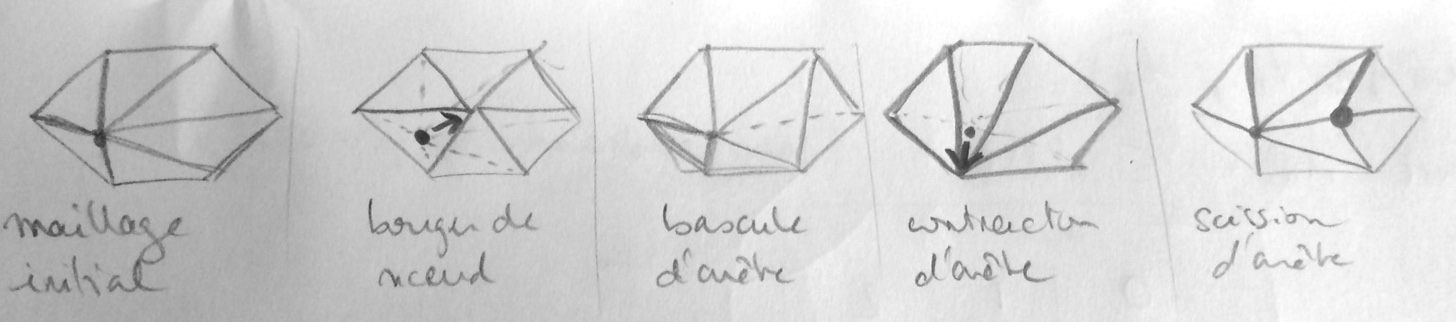
\includegraphics[width=\textwidth]{operations_locales_optimisation_maillage}
\caption{\ldots}
\label{fig:operations_locales_optimisation_maillage}
\end{figure}

\begin{enumerate}
	\item bouger de n\oe ud (direct, \ie $xyz$ ou indirect, \ie $uv$)
	\begin{enumerate}
		\item méthodes heuristiques (lissage laplacien, analogies physiques \cite{farhat1998}, interpolation (IDW, RBF, \ldots) \ldots)
		\item lissage basé sur l'optimisation d'une métrique de qualité \cite{freitag1995, canann1998, jiao2008} \cite{gargallo2014} $\to$ maillage supporté sur un carreau de surface paramétrique
	\end{enumerate}
	\item changements locaux de connectivité
	\begin{enumerate}
		\item bascule d'arête
		\item contraction d'arête
		\item scission d'arête
	\end{enumerate}
\end{enumerate}

%Dans cette thèse,
%\begin{enumerate}
%	\item (\autoref{item:methodo_bodyfitted_ALE})/de nombreux codes de calculs ne tolèrent pas les changement de connectivité en cours de calcul $\Rightarrow$ on se concentre essentiellement sur le bouger de n\oe ud (déformation pure) 
%	\item on n'effectuera des reconnections locales qu'en dernier recours (remaillage)
%\end{enumerate}



\par\bigskip
le maillage doit être une approximation géométrique fidèle de l’interface (dont la géométrie
« exacte » est définie par le modèle BRep)\\
$\to$ solution la plus simple : le maillage interpole la surface \brep\ aux n\oe uds (qui sont alors localisés sur des entités \brep\ et donc sur un ou plusieurs carreaux de surface) $\Rightarrow$ l'écart de corde doit être contrôlé (taille d'élément dicté par le rayon de courbure local, maillage explicite des caractéristiques/singularités géométriques (arêtes vives, coins, \ldots))


\section{Lien entre modèle \brep\ et maillage trans-carreaux}
Objectifs :
\begin{enumerate}
	\item alléger les contraintes sur le maillage inutilement imposées par la topologie du modèle \brep (arêtes douces)
	\item représenter fidèlement 
\end{enumerate}

\subsection{Construction d'une structure d'hypergraphe}


\section{Déformation de maillage trans-carreaux basé sur un modèle \brep\ dynamique}
\subsection{Correspondance d'hypergraphes}

\subsection{Régénération du maillage contraint}

\subsection{\anglais{Untanglement}}

\subsection{Optimisation par bouger de n\oe ud}
\label{section:projection_surface_composite}

\subsection{Optimisation par reconnections locales}
\subsubsection{Bascule d'arête}
Les arêtes contenues dans les chaînes ne peuvent pas être basculées.

\subsubsection{Contraction d'arête}
Soit $e$ l'arête entre les n\oe uds $p_1$ et $p_2$. Sans restreindre la généralité, on supposera que $\ddl(p_1) \leq 
\ddl(p_2)$.
Ici, $\ddl(p)$ représente le nombre de degrés de liberté du n\oe ud $n$, \ie 
\begin{itemize}
	\item $\ddl(p) = 0$ si $n$ est contraint sur un sommet \brep\ ;
	\item $\ddl(p) = 1$ si $n$ est contraint sur une hyper-arête (chaîne) ;
	\item $\ddl(p) = 2$ si $n$ n'est pas contraint.
\end{itemize}
Si $\ddl(p_1) = \ddl(p_2) = 1$, la contraction n'est possible que si $e$ fait partie d'une chaîne, \ie les n\oe uds $p_1$ et $p_2$ sont contraints sur la même hyper-arête (voir \autoref{fig:contraction_arete_cas_1_1}).

\setlength{\imagewidth}{50mm}
\begin{figure}
  \centering
  %
  \hspace*{\fill}
  \subbottom[L'arête $e_2$ peut être contractée, mais pas $e_1$ puisque ses extrémités sont contenues dans deux chaînes distinctes (en rouge et vert).]{
	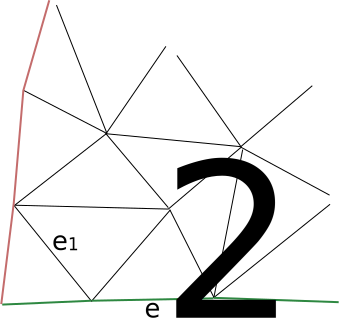
\includegraphics[width=\imagewidth]{contraction_arete_cas_1_1_avant}
	\label{fig:contraction_arete_cas_1_1_avant}
  }
  \hfill%
  \subbottom[Maillage résultant de la contraction de l'arête $e_2$.]{
	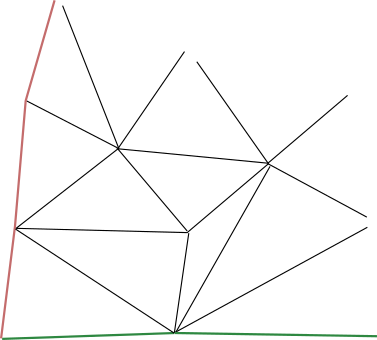
\includegraphics[width=\imagewidth]{contraction_arete_cas_1_1_apres}
	\label{fig:contraction_arete_cas_1_1_apres}
  }
  \hspace*{\fill}
  \caption{Deux cas possibles pour une arête dont les deux sommets ont un seul degré de liberté.}
  \label{fig:contraction_arete_cas_1_1}
  %
\end{figure}

Si $\ddl(p_1) < \ddl(p_2)$ on contracte $e$ vers le n\oe ud $p_1$. 
Si $\ddl(p_1) = \ddl(p_2)$ on contracte $e$ vers son milieu. Afin de localiser précisément ce milieu sur la surface \brep\ (\ie connaître l'entité \brep\ qui le supporte, et ses coordonnées paramétriques dans les carreaux de surface concernés), on l'obtient en calculant la projection sur la surface \brep\ du n\oe ud $p_1$ translaté d'un vecteur $\frac{p_2 - p_1}{2}$, en suivant la procédure décrite dans la \autoref{section:projection_surface_composite}.


\subsubsection{Scission d'arête}
On insère un n\oe ud au milieu d'une arête. Comme pour la contraction d'arête, les coordonnées de ce milieu sont une nouvelle fois obtenue par la procédure de projection décrite dans la \autoref{section:projection_surface_composite}.
Cette fois, la projection du déplacement se fait en partant du sommet de l'arête ayant le plus grand nombre de degrés de liberté.







%%%%%%%%%%%%%%%%%


%% ANNEXES %%
\appendix


%%%%%%%%%%%%%%%%%



%% BIBLIOGRAPHIE %%
\backmatter
\cleardoublepage
\phantomsection
\nocite{*}% à retirer à la fin!!!
\bibliographystyle{mybibstyle}
\bibliography{biblio/spectral_chebyshev,biblio/mesh_generation,biblio/mesh_optimization,biblio/cad,biblio/deformable_geometry,biblio/interface_propagation,biblio/intersection}
%%%%%%%%%%%%%%%%%


\end{document}
